% !TeX spellcheck = cs_CZ
\documentclass[czech,master,dept460,male,csharp,cpdeclaration]{diploma}

\usepackage[autostyle=true,czech=quotes]{csquotes} % korektni sazba uvozovek, podpora pro balik biblatex
\usepackage[backend=bibtex, style=iso-numeric, alldates=iso]{biblatex} % bibliografie
\usepackage{dcolumn} % sloupce tabulky s ciselnymi hodnotami
\usepackage{subfig} % makra pro "podobrazky" a "podtabulky"
\usepackage{rotating}

\usepackage{geometry}
\usepackage{listings}

%\usepackage{mathtools} %- blokuje list obrázků a tabulek

\ThesisAuthor{Bc. Jan Jedlička}

\ThesisSupervisor{prof. Ing. Michal Krátký, Ph.D.}

\CzechThesisTitle{Key-value databázové systémy}

\EnglishThesisTitle{Key-value database systems}

\SubmissionYear{2023}

\ThesisAssignmentFileName{ThesisSpecification_JED0050_vsboee2302B326.pdf}

\Acknowledgement{TODO poděkování}

\CzechAbstract{Cílem diplomové práce je popsat Key-value databázové systémy, ukázat výhodo těchto systémů a představit jedny z jejich významných představitelů. Součástí práce je návrh a implementace testovacího prostředí pro testování těchto systémů s ostatnímy SŘBD. Práce je zakončena vyhodnocením výsledků testů vybraných databázových systémů.}

\CzechKeywords{NoSQL; Key-value databáze}

\EnglishAbstract{The aim of the diploma thesis is to describe Key-value database systems, to show the advantage of these systems and to present some of their important representatives. Part of the work is the design and implementation of a test environment for testing these systems with other DBMS. The work is finished with an evaluation of the test results of selected database systems.}

\EnglishKeywords{NoSQL; Key-value database}

\AddAcronym{NoSQL}{Not only Structured Query Language}
\AddAcronym{Key-value database}{Klíč-hodnota databáze}
\AddAcronym{TTL}{Time to live}
\AddAcronym{YCSB}{Yahoo! Cloud Serving Benchmark}

\addbibresource{citace.bib}

\begin{document}
	
	\MakeTitlePages
	
	\listoffigures
	\listoftables
	
	\chapter{Úvod}
	
	NoSQL Key-value (neboli Klíč-hodnota) databáze~\cite{wiki-key-value-db, ytb-nosql-db} je jedno z paradigmat pro úložiště dat. Databáze je navržena pro ukládání, načítání a správu různých datových struktur, dnes známých jako slovníky nebo hashovací tabulky. Slovníky obsahují kolekci objektů či záznamů, které mohou opět obsahovat množinu různých polí s daty. Záznamy jsou do slovníků, či hashovacích tabulek, ukládána za pomoci klíče, který identifikuje pozici záznamu v datové struktuře a používá se k následnému vyhledávání dat v databázi.
	
	Key-value databáze fungují velice odlišně než tradiční relační databázové systémy. Relační databáze mají předdefinovanou datovou strukturu v databázi jako sérii tabulek s dopředu definovanými datovými typy. Díky tomuto modelu může relační databázový systém provádět řadu optimalizací. Na druhou stranu Key-value databázové systémy mohou mít pro každý záznam různě definované kolekce dat s odlišnými velikostmi a počty atributů. Tato vlastnost nabízí Key-value databázovým systémům flexibilitu a možnost přiblížení se k objektově orientovanému programování. Protože Key-value databáze nevyžaduje pevně nastavené datové typy hodnot, jako je tomu u relační databáze, tak Key-value databáze často potřebují méně paměti k uložení stejných dat, což může vést k značnému nárůstu výkonu. Dále tyto databáze bývají distribuované a dosahují horizontální až lineární škálovatelnosti.
	
	Výkon a nedostatečná standardizace omezovaly Key-value databázové systémy pouze na specializovaná využití, ale díky rychlému přechodu na cloud computing dochází v posledních letech k rozšíření obecné využitelnosti NoSQL databázových systémů. Například databázový systém Redis~\cite{redis} je v současnosti jedním z deseti nejlépe hodnocených~\cite{db-engineers-ranking} databázových systémů napříč relačními i NoSQL databázovými systémy.
	
	\chapter{NoSQL Key-value databázové systémy\label{chapter:no-sql-ky-sys}}
	
	V současné době existuje nespočet různých Key-value databázových systémů, od malých open source projektů po velké placené cloud služby. Různé systém disponují odlišnými vlastnostmi jako je propustnost, škálovatelnost, uživatelská přívětivost skrz dotazovací jazyk a podporu aj. Dle průzkumu~\cite{predictiveanalyticstoday,g2,db-engineers-ranking} bylo vybráno 8 aktuálně významných Key-value databázových systémů se snahou o jednoduchý popis, porovnání (\ref{tab_kvdb_compare}) a konečný výběr vhodných Key-value databázových systémů se snahou otestovat vlastnosti těchto systémů.
	
	\section{Amazon DynamoDB}
	
	Amazon DynamoDB~\cite{dynamodb} je v současné době největší a nejvyužívanější Key-value databázový systém. Jedná se o serverless cloud systém s odezvou v řádu jednotek mikrosekund a využitím v oblastech jako je web tech, IoT, mobile a gaming. DynamoDB je plně a automaticky spravovatelná, multi master databáze zaměřené na vysoké využití horizontální škálovatelnosti. Unikátní primární klíče umožňují identifikaci jednotlivých záznamů v tabulkách a sekundární index zlepšuje dotazovací flexibilitu. Primární klíč je jako vstup do hashovací funkce a výsledný hash nám udává fyzickou pozici uloženého záznamu. DynamoDB poskytuje silnou konzistenci na čtení hodnot od posledních aktualizací. Atomické čítače umožňují automatické změny hodnot číselných atributů. Využívá TTL pro prošlé záznamy v tabulkách. Archivace dat je umožněna díky full backupu. Amazon DynamoDB má i VPC pro soukromou komunikaci bez potřeby využití internetu.
	
	Databázový systém má konzolové API pro správu databáze a práci s daty, systém však nabízí i možnost využití jazyku PartiQL~\cite{partiql} který je vhodný pro kompatibilní SQL dotazy na schema-less databázích. DynamoDB API je rozděleno do čtyř hlavních částí. Kontrolní plán, který zahrnuje funkce spojené s vytvářením, upravováním, mazáním a získáním jmen všech tabulek. Dále umožňuje výpis podrobných specifikací dané tabulky, jako jsou primární klíče, indexy a nastavení propustnosti. Následuje datový plán, který poskytuje CRUD operace pro data v dané tabulce. S daty je možno pracovat jednotlivě po záznamech a nebo pomocí Batch funkcí, které nám dovolují provést stejnou operaci nad desítkami záznamů v jednu chvíli a dosahují tak vyšší propustnosti než při volání stejných funkcí pro jednotlivé záznamy opakovaně. Následně je možná provést Scan pro získání všech záznamů dané tabulky nebo indexu případně Query pro obdržení hledané části dat. Třetí část je DynamoDB Streams pro práci s časovými sekvencemi a práci s logy za posledních 24 hodin. Stream API poskytuje funkce pro výpis všech streamů, konkrétní popis daného streamu, získání iterátoru pro daný stream a nakonec získání jednoho záznamu z daného streamu. A poslední částí API jsou ACID transakce. Transakce jsou rozděleny do dvou částí, první část je určena pro batch vkládání, úpravu a mazání záznamů a druhá část slouží k batch získání záznamů.
		
	\section{Oracle NoSQL Database}
	
	Oracle NoSQL Database~\cite{oraclenosqldb} je databázová cloud služba vhodná pro práci s velkými objemy dat a odhadovatelnou nízkou odezvou v řádu jednotek milisekund. Služba je postavena na enginu z Oracle Berkeley DB. Databáze je plně spravovatelná, flexibilní, škáluje horizontálně, dynamicky a dosahuje vysokých výkonů. Mimo Key-value data se jedná i o spolehlivé úložiště pro dokumenty a data s pevně daným schématem. Vzhledem k tomu že databázový systém je plně spravovaný společností Oracle, tak je pro vývojáře rychlé a snadné začít tuto službu využívat a soustředit se pouze na vývoj aplikací, neboť není potřeba se obtěžovat se správou základní infrastruktury databáze, softwaru, zabezpečení atp. Jedná se o Single Master, Multi Replica grafový systém. Pokud dojde k chybě na masteru, je master automaticky nahrazen jednou z replik. Pro Key-value ukládání s kapacitu jednotek terabytů využívá systém velký počet Storage uzlů, které je možno skupinově konfigurovat. Pro udržení konzistence jsou Storage uzly replikovány. Uzly a hrany v grafu reprezentují entity které vytvářejí vztahy a propojení. Sdílený systém, uniformně alokuje data okolo ostatních částí skupin. Databáze obsahuje i SQL Query s jazykem pro import, export a přenos dat mezi různými Oracle NoSQL databázemi. Mimo jiné je zde podpora i pro Failover, SwitchOver, Bulk Get API, Off Heap Cache a podpora Big Data SQL.
	
	Restové API pro Oracle NoSQL Database je rozděleno do pěti částí. Správa indexů, která dovoluje vytvářet a mazat indexy pro danou tabulku. Tato část API také umožňuje zobrazit všechny indexy které jsou pro danou tabulku vytvořeny a společně s detailním popisem každého indexu. Druhá část API se věnuje dotazům, umožňuje tedy syntaktickou kontrolu daného SQL dotazu, před připravení a spuštění dotazu. Třetí část je zaměřena na správu záznamů, obsahuje tedy CRUD funkce pro jednotlivé záznamy. Tato část ale neobsahuje funkci pro úpravu existujícího záznamu a ani neumožňuje správu mnoha záznamů najednou, pro úpravu je tedy nutno provést funkci odstranění záznamu a vložení nového a všechny záznamy je tedy také potřeba spravovat jednotlivě a postupně. Čtvrtá část je zaměřena správě tabulek, obsahuje možnost vytvoření, upravování, a mazání tabulek. Tato část také umožňuje výpis všech tabulek, informace o dané tabulce a využívání dané tabulky. Poslední část API se věnuje správě pracovních požadavků, lze zde zobrazit stav jednotlivých požadavků, mazat požadavky, získat chyby či log daného požadavku a list všech požadavků.
		
	\section{Redis} \label{lab-redis}
	
	Redis~\cite{redis} je in-memory úložiště pro datové struktury, využívané jako Key-value databáze, cache, streaming engine nebo zprostředkovávatel zpráv. Toto datové úložiště má skvělé využití pro klíče v podobě hashe a hodnoty jako velký json objekt. Pro persistenci dat můžeme ukládání dat na disk provádět po nastavitelných pravidelných intervalech, nebo je možné data logovat vždy při vykonávání operací, pokud nemáme zájem o trvanlivost dat je možné ukládání dat vypnout úplně a datové úložiště využít čistě jako cache. Úložiště škáluje horizontálně. Redis podporuje datové struktury jako řetězce, hashe, listy, množiny, bitmapy, hyperloglog a geospatial indexy. Nad datovými typy Redis umožňuje rychlé atomické operace jako rozšíření řetězců, přidání prvků na začátek a konec listů atd. Datové úložiště také poskytuje seřazené množiny pro vytváření indexů dle ID nebo jiného číselného atributu. Redis hashing ukládá data jako klíč a mapu. Keyspace notifikace dovoluje klientům odebírat Publisher-Subscriber kanály. Pro práci s dotazy na souřadnice a geometrii je možné využívat Geo API. Redis umožňuje provádět transakce, volat lua skripty a nastavovat různé úrovně TTL pro záznamy. Redis podporuje Trivial-to-setup Master-Slave asynchronního replikování, společně s rychlou neblokující se prvotní synchronizaci. Struktura pro ukládání dat je Single-rooted replikovaný strom. Redis má vlastní API pro práci s daty pro populární programovací jazyky jako C, Python, Java a Javascript.
	
	S Redis databází lze pracovat například pomocí konzolového rozhraní, toto CLI~\cite{rediscli} poskytuje řadu jednoduše čitelných ale netradičních příkazů pro práci s daty. Vždy potřebujeme specifikovat klíč s jehož daty chceme v databázi pracovat. Pomocí příkazu SET a DEL vkládáme  do databáze či mažeme jednotlivé hodnoty pro zvolený klíč. Příkazem GET získáme hodnoty pro daný klíč, případně můžeme zjistit zda již existuje záznam pro daný klíč příkazem EXISTS. Pokud vyžadujeme práci s poli tak můžeme pro daný klíč zleva i zprava vkládat hodnoty zřetězené v poli díky příkazům LPUSH a RPUSH. Obdobně odebíráme hodnoty z pole pomocí LPOP a RPOP, příkazem LRANGE vypíšeme hodnoty z pole a příkazem LLEN zjistíme počet jeho záznamů. Místo jednoduchých polí je možno pracovat i s množinami pomocí příkazů SADD, SREM, SISMEMBER a obdobně, množiny mohou být i seřazené a pro ně se využívají příkazy jako ZADD. Pro práci se záznamy strukturovaných jako kolekce párů atribut-hodnota se využívá datový typ Hash, umožňuje nám pro daný klíč uložit záznam obsahující názvy atributů a jednotlivé hodnoty pro ně. Opět se zde využívají příkazy jako HSET a HGETALL pro nastavení a získání daného záznamu, případně HGET pro získání hodnoty daného atributu pro záznam na zadaném klíči. API obsahuje také příkazy pro ostatní datové typy jako jsou Bitmapy, Geo prostory, HyperLogLog a další.
	
	\section{Aerospike} \label{lab-aerospike}
	
	Aerospike~\cite{aerospike} je Key-value databáze využívající Hybrid Memory architekturu~\cite{hybmem-arch}, která umožňuje odezvu do jednotek milisekund a vysokou propustnost v řádu stovek tisíc až milionu operací za sekundu. Hybrid Memory architektura od Aerospike je implementována tak, že index je čistě In-Memory, tím pádem není index perzistentní (vhodné například pro uživatelské cache sessions), a data jsou uložena čistě perzistentně na SSD disku a čtou se přímo z něj. Díky tomu že je Aerospike jako Key-value databáze naprosto Schena-less tak je možné definovat Sets a Bins za běhu pro maximální flexibilitu aplikací. Databáze škáluje lineárně a poskytuje silnou konzistenci, nízkou cenu a korektnost. Umožňuje real-time analýzu pro rychlé rozhodování a dynamickou optimalizaci pro vhodné využívání zdrojů dat, proto je databáze vhodná pro velké a stále aktualizované databáze. Poskytuje server-side clustering, bezpečnost na transportní vrstvě. Databáze také umožňuje Customer deployment s nulovým downtime. V praxi se Aerospike díky svým vlastnostem využívá například pro banking, telekomunikace, adtech a gaming. Aerospike poskytuje vlastní silný dotazovací jazyk AQL~\cite{aql}, který má prakticky shodnou syntaxi jako SQL (i když se o SQL nejedná). Vlastní vytvořitelné agregační funkce pomocí Lua jazyku (flexibilní pro agregační algoritmy).
	
	Dotazovací jazyk AQL se snaží zachovat standardní SQL syntaxi, obvyklé příkazy SELECT, INSERT, DELETE jsou tedy zachovány. Je možné i vytvářet vlastní indexy nad tabulkami pomocí CREATE INDEX a provádět agregace pomocí AGGREGATE. Pro dotazy nad konkrétním záznamem specifikovaným pomocí hexadecimálního řetězce či Base64 lze v podmínce dotazu použít porovnání hodnoty s DIGEST nebo EDIGEST. Dotazování můžeme provádět i standardně nad primárním klíčem a ostatními atributy. Při vkládání záznamů lze specifikovat speciální datové typy atributů jako je LIST, MAP, GEOJSON a další.
	
	\section{Oracle Berkeley DB}
	
	Oracle Berkeley DB~\cite{berkeleydb} je rodina vestavěných Key-value databázových knihoven. Jedná se o čistě In-memory databázi, díky čemuž dosahuje vysokého výkonu a odezvy v jednotkách mikrosekund. Databáze škáluje horizontálně. Data jsou replikována pro vysokou dostupnost z vícero zdrojů a dobrou toleranci chybovosti. Oracle Berkeley DB využívá vhodné datové struktury pro práci s daty jako je B-strom, hash table indexy nebo fronta. Databáze využívá obnovitelné ACID transakce a poskytuje několik různých úrovní izolace (včetně MVCC~\cite{mvcc}). Data jsou dělena do oddílů dle key ranges. Umožňuje komprimaci dat. Databáze je Single-master, Multi-replica, tedy je vysoce dostupná a umožňuje dobrou konfigurovatelnost. Repliky umožňují čtecí škálovatelnost, rychlý fail-over, hot-standby a další distribuované konfigurace dodávající podnikové prostředky v malém, vestavěném balíčku. Pro přístup k datům a nastavení databáze se využívá jednoduché volání funcion-call API. Spousta moderních programovacích jazyků, jako například C++, C\#, Javy, Python atp. podporuje tyto knihovny. Data mohou být ukládána v nativním formátu aplikace, XML, SQL nebo jako Java Objekty. Oracle Berkeley DB je vhodný nástroj pro vše od lokálního úložiště po world-wide distribuovanou databáze (od kilobytů po petabyty).
	
	Interakce s Berkley DB SQL API je prakticky identická jako s SQLite~\cite{sqlite}. Pro práci s databází vytvořenou rozhraním BDB SQL používáte stejná rozhraní API, stejné Shell prostředí, stejné příkazy SQL a stejné PRAGMA, jako se využívá u SQLite. BDB SQL rozšiřuje standardní SQLite PRAGMA o možnosti nastavení velikosti alokované paměti sdílených zdrojů, nastavení počtu bucketů v hashovací tabulce objektů zámků, zvolení soukromého prostředí místo sdíleného, přesměrování logování chyb do vlastního souboru, nastavení příznaku, který způsobí, že sdílené prostředky databáze budou vytvořeny ve sdílené paměti systému a další. Dalším drobným rozdílem je že BDB SQL rozhraní nepodporuje klíčové slovo IMMEDIATE.
	
	\section{Riak KV} \label{lab-riak}
	
	Riak KV~\cite{riak} je distribuovaná NoSQL Key-value databáze s pokročilou lokání a multi-cluster replikací, která garantuje čtení a zápis i v případě selhání hardwaru nebo síťových oddílů. Riak využívá bezkonfliktní replikované datové typy (CRDT~\cite{crdt}), které umožňují nezávisle a souběžně aktualizovat jakoukoliv repliku v distribuované databázi se zajištěním sjednocení hodnot pomocí algoritmu který je součásti samotného datového typu (flagy, registry, čítače, množiny a mapy). Poskytuje konfiguraci aktivního clusteru a dosahuje nízké latence v řádu jednotek milisekund díky dodávání dat z nejbližšího data centra. Databáze rozděluje data z clusterů pro své dostupné zóny, má multi cluster repliky a využívá redundance dat v geografickém regionu. Riak tedy automaticky distribuuje data skrz cluster, pro robustnost a vysoký výkon. Key-value databáze poskytuje flexibilní datový model bez předem definovaného schématu. Databáze vylepšené logování chyb a reporty. Data jsou automaticky komprimována pomocí Snappy kompresní knihovny~\cite{snappy}. Databáze využívá master-less architekturu, je vysoce dostupná a má design horizontální škálovatelnosti. Škálovatelnost je téměř lineární při využití snadného přidání hardwarové kapacity bez nutnosti mnoha operací. Riak KV dovoluje zpracování dat pro analýzu a vyvození závěrů pro zlepšení chodu databáze. Riak KV je navržen pro nulové restrikce na hodnoty, takže session data mohou být enkódována mnoha způsoby a nevyžadují změnu schématu. Během nejvyšší zátěže nezhoršuje databáze zápis a horizontální škálovatelnost, uživatelé jsou stále obsluhování bez problémů. Databáze je vhodná pro ukládání velkého množství nestrukturovaných dat, také pro big-data aplikace, ukládání dat z připojených zařízení a replikování dat do okolí. Díky nízké latency je databáze vhodná i pro chat/messaging aplikace. Riak KV exceluje v soukromém, veřejném či hybridním cloud nasazování.
	
	Riak KV API obsahuje všechny potřebné CRUD operace pro správu objektů. Při vytváření nových objektů je potřeba nastavit typ a název bucketu, který skladuje klíče a data do něj vložená, bucket má také vlastní indexy pro vyhledávání dat uvnitř něj. Dva různé buckety mohou uchovávat stejnou hodnotu klíče, ale jeden bucket obsahuje pouze unikátní klíče. Klíč pro data lze specifikovat explicitně vlastní při vytváření objektu pomocí parametru nebo při jeho absenci je datům přiřazen klíč náhodný. Při vkládání dat do databáze můžeme jednoduše nastavit parametr TTL daného objektu a také počet jeho replik. Při čtení dat můžeme před získáním výsledku zadat minimální počet replik, které se musí shodnout na stejných datech pro zvolený klíč. Pro efektivnější dotazy lze vytvořit vlastní indexy pro výchozí nebo námi zvolené datové schéma. Lze se dotazovat na data pro zvolený klíč nebo provádět fulltextové vyhledávání. Databáze poskytuje i funkce pro tvorbu sekundárních indexů a následné dotazy nad nimi. Riak API také umožňuje hlubší nastavení autorizace a bezpečnosti, práce s replikami a řešení konfliktů.
	
	\section{Voldemort}
	
	Project Voldemort~\cite{voldemort} je distribuovaná Key-value databáze založena na Amazon DynamoDB. Škáluje horizontálně pro čtení i zápisu. Umožňuje zapojení storage-enginu (MySQL, Read-Only). Databáze automaticky replikuje data napříč servery pro dostupnost a bezpečnost jednotlivých oddílů při vysoké propustnosti, nicméně každý server obsahuje pouze část z celkových dat. Databáze je decentralizovaná z pohledu uzlů, každý uzel je samostatný a nezávislý, nenachází se zde žádný centrální řídící uzel nebo uzel řídící řešení chyb. Voldemort má výkonost desítek tisíc operací za sekundu na jeden uzel (1 op. za 50 mikrosekund), samozřejmě závisí na hardwaru, síti, systému disku atp. Konzistence dat je nastavitelná (přísné kvórum nebo případná konzistence). Selhání serverů jsou ošetřována transparentně, pro lepší viditelnost, interní monitorování a validaci dat lze využívat JMX~\cite{jmx}. Data jsou verzována pro maximální integritu i během poruch. In-Memory caching pro eliminaci oddělených částí cache, jednoduché a rychlé in-memory testování (např. pro unit testy). Databáze umožňuje jednoduchou distribuci dat skrz stroje, data mohou být rozdělována například dle primárních klíčů. Databáze má hashovatelné schéma, vyhledávání dle primárního klíče a možnost modifikace jednotlivých hodnot. Voldemort poskytuje široké možnosti pro klíče i hodnoty díky serializaci včetně listů a tuplů s pojmenovanými poli. Pro serializaci (Java Serialization, Thrift, Avro) se využívá JSON datový model v kompaktním bytovém formátu, probíhá zde typová kontrola dat dle očekávaného schématu. Pomocí API je možné rozhodovat o replikování a místech ukládání dat, nastavení různé strategie pro specifické aplikace a možnost distribuce dat skrz data centra která jsou mezi sebou geologicky velice vzdálená. Databáze neposkytuje triggery, cizí klíče ani komplexní filtry pro dotazy.
	
	Práce s Voldemort databází z pohledu klienta je přímočará, API se skládá pouze z pár základních funkcí pro správu dat. Tyto funkce jsou Put, Get a Del pro nastavení, získání a odstranění hodnot pro explicitně specifikovaný klíč. Funkce GetAll umožňuje obdržet více hodnot pro více specifikovaných klíčů pomocí volání pouze jedné funkce, GetAll dosahuje vyšší propustnosti než zřetězené volání samostatné funkce Get. Pro připojení k Voldemort databázi a nastavení výchozího uzlu úložiště se využívá funkce Bootstrap, bez nastavení výchozího uzlu je potřeba specifikovat uzel explicitně před každým volání funkce Get a dalších. Pro funkci Bootstrap je také možné nastavovat serializer pro klíče i hodnoty, čas spojení klienta se serverem a interval automatické změny uzlu v rámci clusteru na ten nejvhodnější. Pro ukončení komunikace se využívá jednoduše funkce Close.
	
	\section{InfinityDB}
	
	InfinityDB~\cite{infinitydb} je NoSQL hierarchicky tříděná Key-value databáze implementovaná v Javě. Databáze má možnost využít čistě In-Memory ukládání dat která je vhodné pro cache, nebo naopak se mohou data ukládat i perzistentně na disk do souboru, nastavení měnit bez zasahování do kódu. Přístup k datům v cachy je plně více vláknový, vyžívá se většina jader, a data která nejsou často využívaná jsou stránkována na disk. Výkon v jednotkách miliónů operací za sekundu pro více vláknové operace v cachy. Veškerá data a informace o databázi jsou na disku uložena v jednom souboru, jsou proto stále aktuální, čímž je docílena maximální bezpečnost, korektnost. Databáze je designovaná právě pro použití jen jednoho kompletního souboru s okamžitým zotavením a nevyžaduje proto administraci. Databáze neobsahuje dodatečné konfigurační nebo dočasné soubory, upgrade skripty a ani logy. Zotavení je tady bez logů o transakcích okamžité ihned po restartu. V databázi není potřeba dělat čištění junk souborů po operacích když zde nejsou žádné zanechány. InfinityDB podporuje ACID pro vlákna a ACD pro bulk operace. Databáze poskytuje prostor pro ukládání strukturovaných, polo strukturovaných a nestrukturovaných dat, tento jednoduchý model umožňuje ukládání vnořených Multi-values, je možné reprezentovat stromy, grafy, Key/Value mapy, dokumenty, velká řídká pole a tabulky. Schema je možné měnit za běhu pro zpětnou i následující kompatibilitu. Data dotazů lze dynamicky sledovat (set logic views, delta views, ranges). Databáze se využívá pro servery, pracovní stanice a příruční zařízení.
	
	InfinityDB poskytuje základní jednoduché API o deseti hlavních API voláních. Funkcionalitu pro vkládání, úpravu a mazání hodnot obstarávají funkce Insert, Update, Delete. Funkce Delete je rozšířena o funkci Delete-suffixes, která umožňuje odstranit vícero hodnot v jednom volání funkce. Pro získávání hodnot se využívá kurzoru jehož pohyb v obou směrech obstarávají funkce First, Next, Last a Previous. A nakonec pro možnost využívání transakcí jsou zde i potřebné funkce Commit a Rollback.

	\begin{sidewaystable}
		\centering
		\caption{Porovnání Key-value databází\label{tab_kvdb_compare}}
		\scalebox{0.8}
		{
			\begin{tabular}{ l|c c c c c c c c } 
				\toprule
				Databáze & Amazon & Oracle & Redis & Aerospike & Oracle & Riak & Voldemort & InfinityDB \\
				& DynamoDB & NoSQL DB & & & Berkeley DB & KV & & \\
				\midrule
				Čistě cloud & ano & ne & ne & ne & ne & ne & ne & ne \\
				Schéma dat & ne & ano i ne & ne & ne & ne & ne & ne & ano \\
				Licence & komerční & open source & open source & open source & open source & open source & open source & komerční \\
				Server OS & hostovaná & Linux, Solaris & Linux, Windows, & Linux & Linux, Windows, & Linux, OS X & Linux, Windows &  Linux, Windows, \\
				& & & OS X, BSD & & OS X, Android ad. & & & OS X, Solaris\\
				Napsáno v & - & Java & C & C & C, C++, Java & Erlang & Java & Java\\
				Sekundární & ano & ano & ano & ano & ano & omezené & ne & ne \\
				indexy & & & & & & & & \\
				Koncept & ACID & ACID & atomické, & atomické & ACID & ne & ne & ACID \\
				transakcí & & v rámci uzlu & izolované & & & & & \\
				Triggery & ano & ne & pub/sub & ne & ano & ano & ne & ne \\
				Dělící & sdílení & sdílení & sdílení & sdílení & ne & sdílení & ne & ne \\ 
				metody \\
				Replikační & ano & source-replica & source-replica, & volitelná & source-replica & volitelný & ne & ne \\
				metody & & multi-region & multi-source & faktor repl. & & faktor repl. \\
				Administrace & vysoká & nízká & vysoká & vysoká & vysoká & vysoká & vysoká & ne\\
				Škálovatelnost & horizontální & horizontální & horizontální & lineární & horizontální & lineární & horizontální & horizontální\\
				Odezva & mikrosekundy & milisekundy & milisekundy & milisekundy & mikrosekundy & milisekundy & milisekundy & milisekundy \\
				Dotazovací & PartiQL & Omezený SQL & Redis & AQL & SQL & Riak & Voldemort & InfinityDB \\
				jazyk & & & query & & & query & query & query \\
				\bottomrule
			\end{tabular}
		}
	\end{sidewaystable}
	
	\section {Nezmíněné významné NoSQL databáze}
	
		Do práce nebyly záměrně zahrnuty databázové systémy MongoDB a Couchbase~\cite{mongodb,couchbase}. I když se jedná o známé a hojně využívané NoSQL databáze, tak byly obě záměrné z práce vynechány protože mají key-value až jako sekundární datový model, primárně jsou určeny pro ukládání dokumentově orientovaných informací~\cite{documentdb}. Další často využívaná a nezmíněná NoSQL databáze je Cassandra~\cite{cassandra}, tato databáze udává jako datový model wide-column store~\cite{widecolumnstore} a proto ze stejného důvodu byla i tato databáze vyřazena z testování.
	
	\chapter{Prostředí pro testování databázových systémů}
	
	Různé databázové systémy mohou k řešení jednotlivých problémů přistupovat odlišně. Pokud chceme rozhodnout, který ze systémů je nejvhodnější pro určité úkoly musíme provést řadu testů a porovnání. Je prakticky nemožné najít ideální databázový systém který bude nejlepší ve všech aspektech pro všechna data a případy využití, testování nám ale odhalí který ze systémů vyniká a naopak zaostává pro konkrétní operace nad konkrétními daty. Proto je zapotřebí najít ideální prostředí pro možnost změření a porovnání vlastností vybraných NoSQL Key-value databázových systémů v Kapitole~\ref{chapter:no-sql-ky-sys}.
	
	Existuje celá řada nástrojů pro měření výkonu databázových systémů. Mezi dva dosti známé a dostupné nástroje se řadí například TPC~\cite{tpc} a YCSB~\cite{ycsb}. TPC benchmarky od Transaction Processing Performance Council se dělí do mnoha kategorií, například TPC-H je považován spíše za benchmark pro systémy pro podporu rozhodování~\cite{dss} a TPCx-BB je benchmark pro Big Data. Obecně se TPC benchmarky využívají spíš pro typické relační databázové systémy. Na druhou stranu Yahoo! Cloud Serving Benchmark (dále jen YCSB) od Yahoo! je open-source specifikace a sada programů pro vyhodnocování možností vyhledávání a údržby počítačových programů. Často se ale právě YCSB používá k porovnání relativního výkonu NoSQL databázových systémů což je pro tuto práci zaměřenou na Key-value databáze ideální a proto i byla tato technologie zvolena pro měření výkonu jednotlivých databázových systémů~\cite{benchmark-pdf-1, benchmark-pdf-2}.
	
	\section{YCSB} \label{lab-ycsb}
	
	YCSB architektura je založená na pluginech a poskytuje snadnou rozšiřitelnost pomocí skriptů. Pro velkou část databázových systémů existuje podpora v podobě bindingů. Samotný benchmark se následně skládá ze dvou částí, loading fáze zaměřená na vložení dat do databáze a running fáze ve které se spustí daný test (\ref{ycsb-blok-schema}).
	
	Při spouštění každého testu je možné nastavit určité parametry pro lepší konkretizaci měřeného scénáře~\cite{ytb-ycsb}. První a druhý parametr slouží pro specifikaci loading nebo running fáze a výběr testovaného databázového sytému. Následně se vybírá testovaná scénář (Workload), počet záznamů v databázi, počet atributů daného záznamu, bytovou velikost každého atributu v záznamu, počet vláken, umístění serveru databáze a nakonec distribuci dotazů (uniformní, exponenciální, sekvenční, nejnovější, hotspot, definované).
	
	YCSB poskytuje 5 různých scénářů označených A až F pro testování propustnosti, odezvy a škálovatelnosti jednotlivých databázových systémů. Tyto pracovní scénáře, neboli Workloads~\cite{benchmark-pdf-1, workloads}, napodobují různé chování požadavků webových aplikací, jako jsou scénáře zaměřeny výhradně na čtení, zápis a nebo i kombinace obojího. Konkrétní počet zvolených operací dle procentuální definice je vypočítán na základě parametru určujícího celkový počet operací daného scénáře. Při sekvenčním skenování ve Workloadu E je maximální počet skenovaných záznamů v jedné operaci definován jako 5\% z celkového počtu záznamů, takže při počtu záznamů 1000 bude každá operace skenování číst právě 1 až 50 záznamů.
	
	\begin{itemize} \label{lab-workloads}
		\item Workload A (Update heavy)
		\begin{itemize}
			\item 50\% operací zaměřených na čtení a 50\% operací zaměřených na vkládání
		\end{itemize}
		\item Workload B (Read mostly)
		\begin{itemize}
			\item 95\% operací zaměřených na čtení a 5\% operací zaměřených na vkládání
		\end{itemize}
		\item Workload C (Read only)
		\begin{itemize}
			\item 100\% operací zaměřených na čtení
		\end{itemize}
		\item Workload D (Read latest)
		\begin{itemize}
			\item 95\% operací zaměřených na čtení, 5\% operací zaměřených na vkládání a poslední vložené záznamy jsou čteny přednostně
		\end{itemize}
		\item Workload E (Short ranges)
		\begin{itemize}
			\item 95\% operací zaměřených na sekvenční skenování nízkého počtu záznamů a 5\% operací zaměřených na vkládání
		\end{itemize}
		\item Workload F (Read-modify-write)
		\begin{itemize}
			\item každá operace se skládá ze čtení daného záznamu, úpravy záznamu a následné vložení změněného záznamu zpět
		\end{itemize}
	\end{itemize}

	\begin{figure}
		\centering
		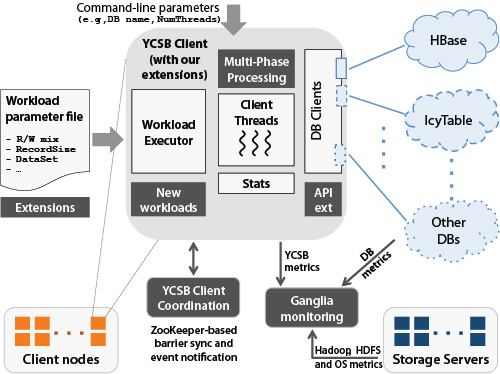
\includegraphics[scale=0.7]{Data/ycsb-1.jpg}
		\caption{YCSB rámec testování funkčnosti \cite{ycsb-parallel-data-lab}\label{ycsb-blok-schema}}
	\end{figure}

	\section{TPC}
	
	Transaction Processing Performance Council~\cite{tpc}, dále jen TPC, je společnost spravující software pro vytváření kvalitních benchmarků výkonnosti systémů pro online zpracování transakcí (OLTP)~\cite{oltp} a i možnosti jejich následného monitoringu a porovnávání. TPC benchmarky poskytují spolehlivé testy pro velké firmy s přiměřenou zátěží, výsledkem benchmarků je počet transakcí za minutu (tpm).
	
	TPC benchmarky jsou rozděleny do vícero modelů pro různě specifikované testy. Prvním z modelů pro OLTP byl TPC Benchmark A (TPC-A), který následně nahradil benchmark TPC-B a aktuálně se v tomto odvětví využívá poslední generace OLTP benchmarků TPC-C a TPC-E. Například modely TPC-DS/DI a TPC-H jsou uzpůsobeny pro benchmark pro systémy pro podporu rozhodování~\cite{dss}. TPC benchmarky jsou přizpůsobeny i pro virtualizaci, IoT~\cite{iot} a další viz tabulka TPC benchmarků (\ref{tab_tpc_modely}).
	
	Model TPC-C~\cite{tpc-c} simuluje velkoobchodní provoz s více sklady, známý jednoduše jako "společnost". V minimálním testu má společnost deset skladů, každý s deseti uživatelskými terminály. Každý sklad obsluhuje deset definovaných prodejních okrsků, každý s 3 000 zákazníky, kteří objednávají podle katalogu výrobků o 100 000 položkách. Nejčastějšími transakcemi jsou objednávky zákazníků, přičemž každá objednávka obsahuje v průměru 10 položek, a platby zákazníků. Méně časté požadavky se dotazují na stav objednávek a skladových zásob, expedují objednávky a doplňují zásoby, které se sníží. Pro testování výkonnosti daného systému se počet skladů zvyšuje tak, aby splňoval požadované minimum potřebné k měření cílové úrovně výkonnosti.
	
	Výsledky srovnávacího testu se měří v transakcích za minutu, známých jako tpmC. První výsledek tpmC byl zveřejněn v září 1992 pro IBM AS/400 a přinesl výsledek 54 tpmC. V roce 2000 byl průměrný výsledek pro špičkové stroje 2,4 milionu tpmC a společnosti ve snaze získat rekord stavěly systémy velmi velkých rozměrů. Současný rekord byl stanoven v roce 2020 pomocí cloud computingu, který poskytl 707,3 milionu tpmC~\cite{tpc-c-top-result}. Nedávné výsledky pro menší lokální systémy se zaměřily na snížení nákladů na tpmC.
	
	\begin{table}
		\centering
		\begin{tabular}{ l | l }
			\toprule
			TPC benchmark & využití\\
			\midrule
			TPC-C, TPC-E & zpracovávání transakcí \\
			TPC-H, TPC-DS, TPC-DI & podpora rozhodování \\
			TPCx-V, TPCx-HCI & virtualizace \\
			TPCx-HS, TPCx-BB & velká data \\
			TPCx-IoT & IoT \\
			TPCx-AI & umělá inteligence \\
			TPC-Energy, TPC-Pricing & běžné specifikace \\
			TPC-A, TPC-B, TPC-APP, TPC-D & zastaralé benchmarky \\
			TPC-R, TPC-W, TPC-VMS & \\
			\bottomrule
		\end{tabular}
		\caption{TPC benchmarky\label{tab_tpc_modely}}
	\end{table}
	
	\chapter{Vyhodnocení výsledků testů}
	
	\section{Testovací prostředí}
	
	Veškeré testy byly spouštěny na vlastním stroji, domácím počítači. Konkrétní specifikace tohoto stroje se nachází v tabulce (\ref{tab_my_pc_spec}). 
	
	\begin{table}
	\centering
	\caption{Specifikace stroje na kterém se spouštěly testy\label{tab_my_pc_spec}}
		\begin{tabular}{ l | l | l } 
			\toprule
			komponent & název & podrobnosti \\
			\midrule
			OS & Microsoft Windows 10 PRO & x64 \\
			CPU & Intel Core i5 4590 & 3,3GHz (Boost 3,7GHz), core/thread 4, Haswell\\
			GPU & NVIDIA GeForce GTX 1660 SUPER & 6GB, 1530MHz (Boost 1785MHz) \\
			RAM & Crucial Ballistix Sport & 8GB (2x4GB), 1600MHz, DDR3 \\
			SSD & Samsung 870 EVO & R/W 560/530MB/s, 1TB, TLC, SATA 6Gb/s \\
			Základní deska & GIGABYTE GA-H81M-H - Intel H81 & 1150 socket, DDR3 DIMM \\
			\bottomrule
		\end{tabular}
	\end{table}

	\section{Zprovoznění testů}
	
	Pro rozsáhlé otestování byly vybrány 4 vhodné Key-value databáze. A to konkrétně Redis (\ref{lab-redis}), Riak KV (\ref{lab-riak}), Aerospike (\ref{lab-aerospike}) a Memcached. Všechny tyto zvolené databáze jsou v aktuálním roce 2024 hodnoceny jako jedny z nejlepších dle žebříčku na webu DB-Engines Ranking~\cite{db-engineers-ranking} právě pro námi testovaný model Key-value. Tento web přiřazuje databázím bodové ohodnocení na základě četnosti nových článků o dané databázi na internetu, obecný zájem, četnosti diskuzí na fórech, množstvím pracovních nabídek a poptávek a relevanci na sociálních sítích.
	
	Ve snaze o možnost testy snadno replikovat, byly všechny databáze instalovány a spouštěny pomocí open-source platformy Docker~\cite{docker}. Proto tedy bylo i zapotřebí najít vhodné a kompatibilní docker images pro každou z testovaných databází. V kontextu této práce Docker pomáhá zrychlit zdlouhavou fázi instalování a nastavení počátečního stavu databází, udržení funkčnosti vybrané verze instalovaného softwaru a odstínění od stavu stroje, na kterém databáze spouštíme.
	
	Veškeré testy byly vytvářeny a spouštěny pomocí frameworku YCSB (\ref{lab-ycsb}). YCSB framework ve své první části Load do databáze vložil data, a následně v druhé části Run spustil testy a vrátil hodnoty výsledků. Pomocí přidání volitelných parametrů bylo možné testy upravit k vlastním potřebám.
	
	Po spuštění databáze v Dockeru se k databázi připojil YCSB framework, který následné prováděl testování nad zvolenou připojenou databází. Pro možnost komunikace bylo zapotřebí zprovoznit YCSB binding pro každou z databází, aby YCSB framework mohl následně úspěšně komunikovat se zvolenou databází, vložit data, spustit testy a vrátit patřičné výsledky.
	
	\section{Popis parametrů testů}
	
	Veškeré testy pro každou z testovaných databází byly spuštěny třikrát, výsledný finální výsledek byl tedy nakonec průměrem ze všech tří testů pro každou databázi v dané testovací kategorii. Každý test byl spouštěn paralelně na čtyřech vláknech.
	
	Do databáze bylo vždy vloženo 100000 záznamů a následující test prováděl 1000000 dotazů nad danou naplněnou databází. Následně byla databáze vyprázdněna, reinstalována a celý proces se následně opakoval ještě dvakrát.
	
	Testy bylo prováděny ve třech YCSB kategoriích. A to Workload A (Update-heavy: 50\% read, 50\% update), Workload B (Read-mostly: 95\% read, 5\% update) a Workload C (Read-only) (\ref{lab-workloads}).
	
	Pro každý Workload a jednotlivé databáze byla vytvořena tabulka výsledků jednotlivých testů a výsledný průměr těchto testů. Mezi nejdůležitější výsledky testů patří celková doba trvání testu, propustnost a 95/99 percentil odezvy na operaci. V tabulce jsou i data o počtu spuštěných operací, průměrné odezvě na operaci, a také minimální a maximální doba odezvy na operaci.
	
	\chapter{Závěr}
	
	TODO
		
	\nocite{*}
	
	\printbibliography[title={Literatura}, heading=bibintoc]
	
\end{document}